\chapter{Kater's Pendulum}

\section*{Objectives}

\begin{enumerate}
\itemsep0em
\item To study the oscillations of a compound pendulum.
\item To find the local value of acceleration due to gravity using a specially designed reversible compound pendulum called Kater's pendulum.  
\end{enumerate}



\section*{Introduction}

\begin{figure}[!htb]
        \centering
        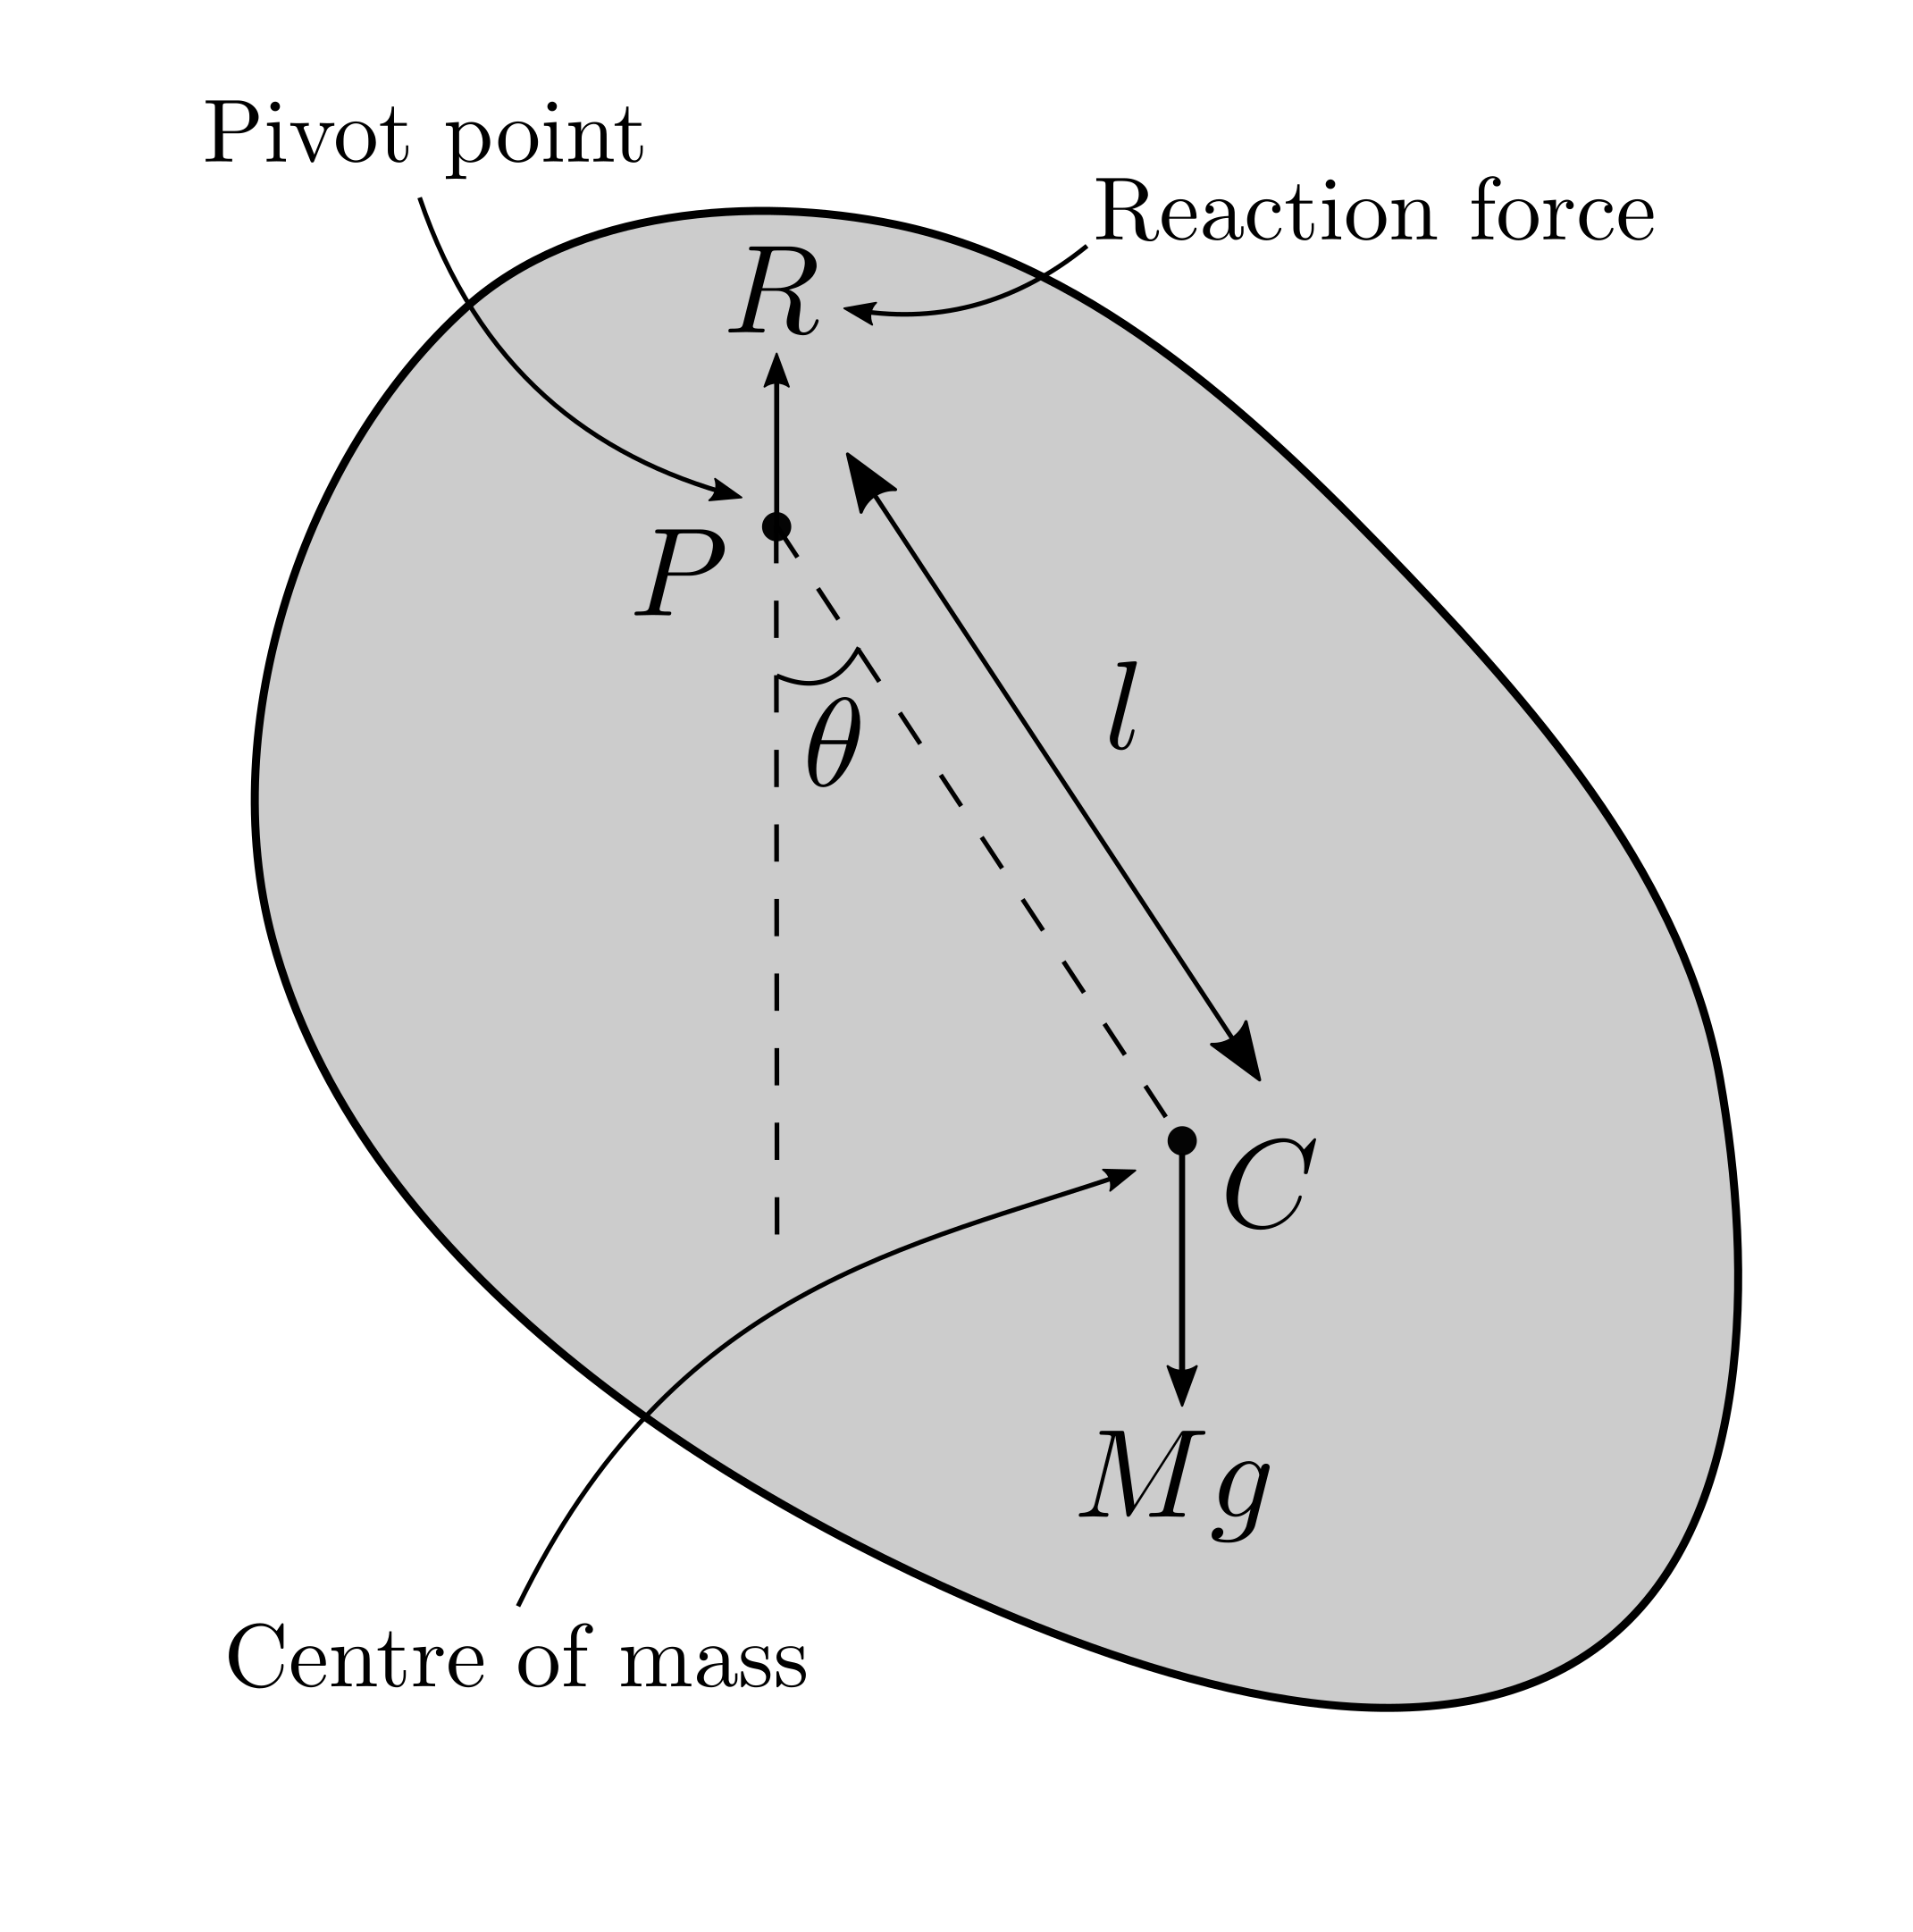
\includegraphics[scale=0.55]{figs/katers-pendulum/compoundPendulum.png}
        \caption{Schematic of a compound pendulum oscillating about a pivot $P$.}
\end{figure}

Kater's pendulum is a compound pendulum that is used to measure the local value of acceleration due to gravity. Before we describe how it does this, it is first important to understand what a compound pendulum is and how it behaves. In its most general sense, a compound pendulum is an extended object whose mass is distributed throughout its body. This is in contrast to a ``simple'' pendulum, where we assume all the mass is concentrated in the oscillating bob. The time period for small oscillations of such a pendulum is given by 
\begin{equation}
    T=2 \pi \sqrt{\frac{I_l}{mgl}},
    \label{eq:Tcomp}
\end{equation}
where $I_l$ is the moment of inertia of the body about the axis of rotation (at $l$), $g$ is acceleration due to gravity, $M$ is the total mass of the body, and $l$ is the distance between the pivot point and the centre of mass. (You should try deriving Equation~(\ref{eq:Tcomp}) using the torque balance equation.) Let $I_\text{CM}$ be the moment of inertia of a body about an axis passing through its centre of mass. By the parallel axis theorem, moment of inertia about any axis parallel to this is
\begin{equation}
    I_l=I_\text{CM}+ml^2,
    \label{parallel-axis-theorem}
\end{equation}
where $l$ is the distance from the centre of mass. $I_\text{CM}$ is usually simply written as $m k^2$, where $k$ is a quantity known as the radius of gyration, and which depends on the configuration of mass and the distance from the parallel axis through the centre of mass, about which the body is rotating. Thus, we have
\begin{equation}
    T = 2 \pi \sqrt{\frac{k^2 + l^2}{gl}}.
    \label{timeperiod-k}
\end{equation}

\begin{question}
\textbf{Question:} Write Equation~(\ref{timeperiod-k}) as a quadratic equation in $l$ (for a given period $T$). What do the roots of this equation correspond to?
\end{question}

From this, it should be clear that there are -- in principle -- an infinite number of points of suspension on a compound pendulum which have the same time period, all of which are at the same distance $l$ from the centre of mass. You can thus imagine drawing a circle of radius $l$ around the centre of mass, and every point on this circle would have the same time period $T_l$. What is less intuitive, however, is that there is a \textsl{second} circle, of radius $k^2/l$, such that all points suspended a distance of $k^2/l$ from the centre of mass \textsl{also} have the same time period $T_l$. There are thus two circles of ``conjugate'' points about which the time period is the same.

\begin{question}
\textbf{Question:} Using Equation~(\ref{timeperiod-k}), show that a point of suspension at a distance $d$ from the centre of mass, and a point of suspension at a distance $k^2/l$ from the centre of mass have the same time period of oscillation.

\textbf{Question:} Now, imagine a one-dimensional rod. Show that there are strictly four points of suspension which produce the same time period of oscillation:
\begin{equation}
    l, \quad -l, \quad \frac{k^2}{l}, \quad -\frac{k^2}{l}.
\end{equation}
Do all of them have to lie on the pendulum? Show that as one point of suspension approach the centre of mass, the other recedes from it.
\end{question}

We can use the Equation~(\ref{eq:Tcomp}) to measure the acceleration due to gravity by simply rearranging it so that 
\begin{equation}
    g=\frac{4\pi^2}{T^2}\frac{I_l}{ml}.
    \label{eq:T1}
\end{equation}

However, to get the value of $g$ from Equation~(\ref{eq:T1}), one has to know its moment of inertia accurately, which requires an accurate calculation of the body's mass distribution. Furthermore, using the formula as it stands requires us to know the position of the centre of mass precisely, since $l$ is measured with respect to this point. Doing this, however, is not easy. Kater's pendulum ingeniously sidesteps both of these problems through its design by depending primarily on the sum of two distances from the centre of mass in opposite directions, with the points between which distance is measured being the easily located knife-edges.

% \begin{question}
% \textbf{Question:} The knife-edges are assumed to have negligible masses. With respect to what do you think they are negligible?
% \end{question}

\section*{Theory}

Kater's Pendulum, shown in Figure~(\ref{fig:katers-setup}), consists of a thick rod (mass $M$) with two knife edges and two unequal masses, $M_1$ and $M_2$. These masses are adjustable; they can be moved along the rod.

 \begin{figure}[!htb]
        \centering
        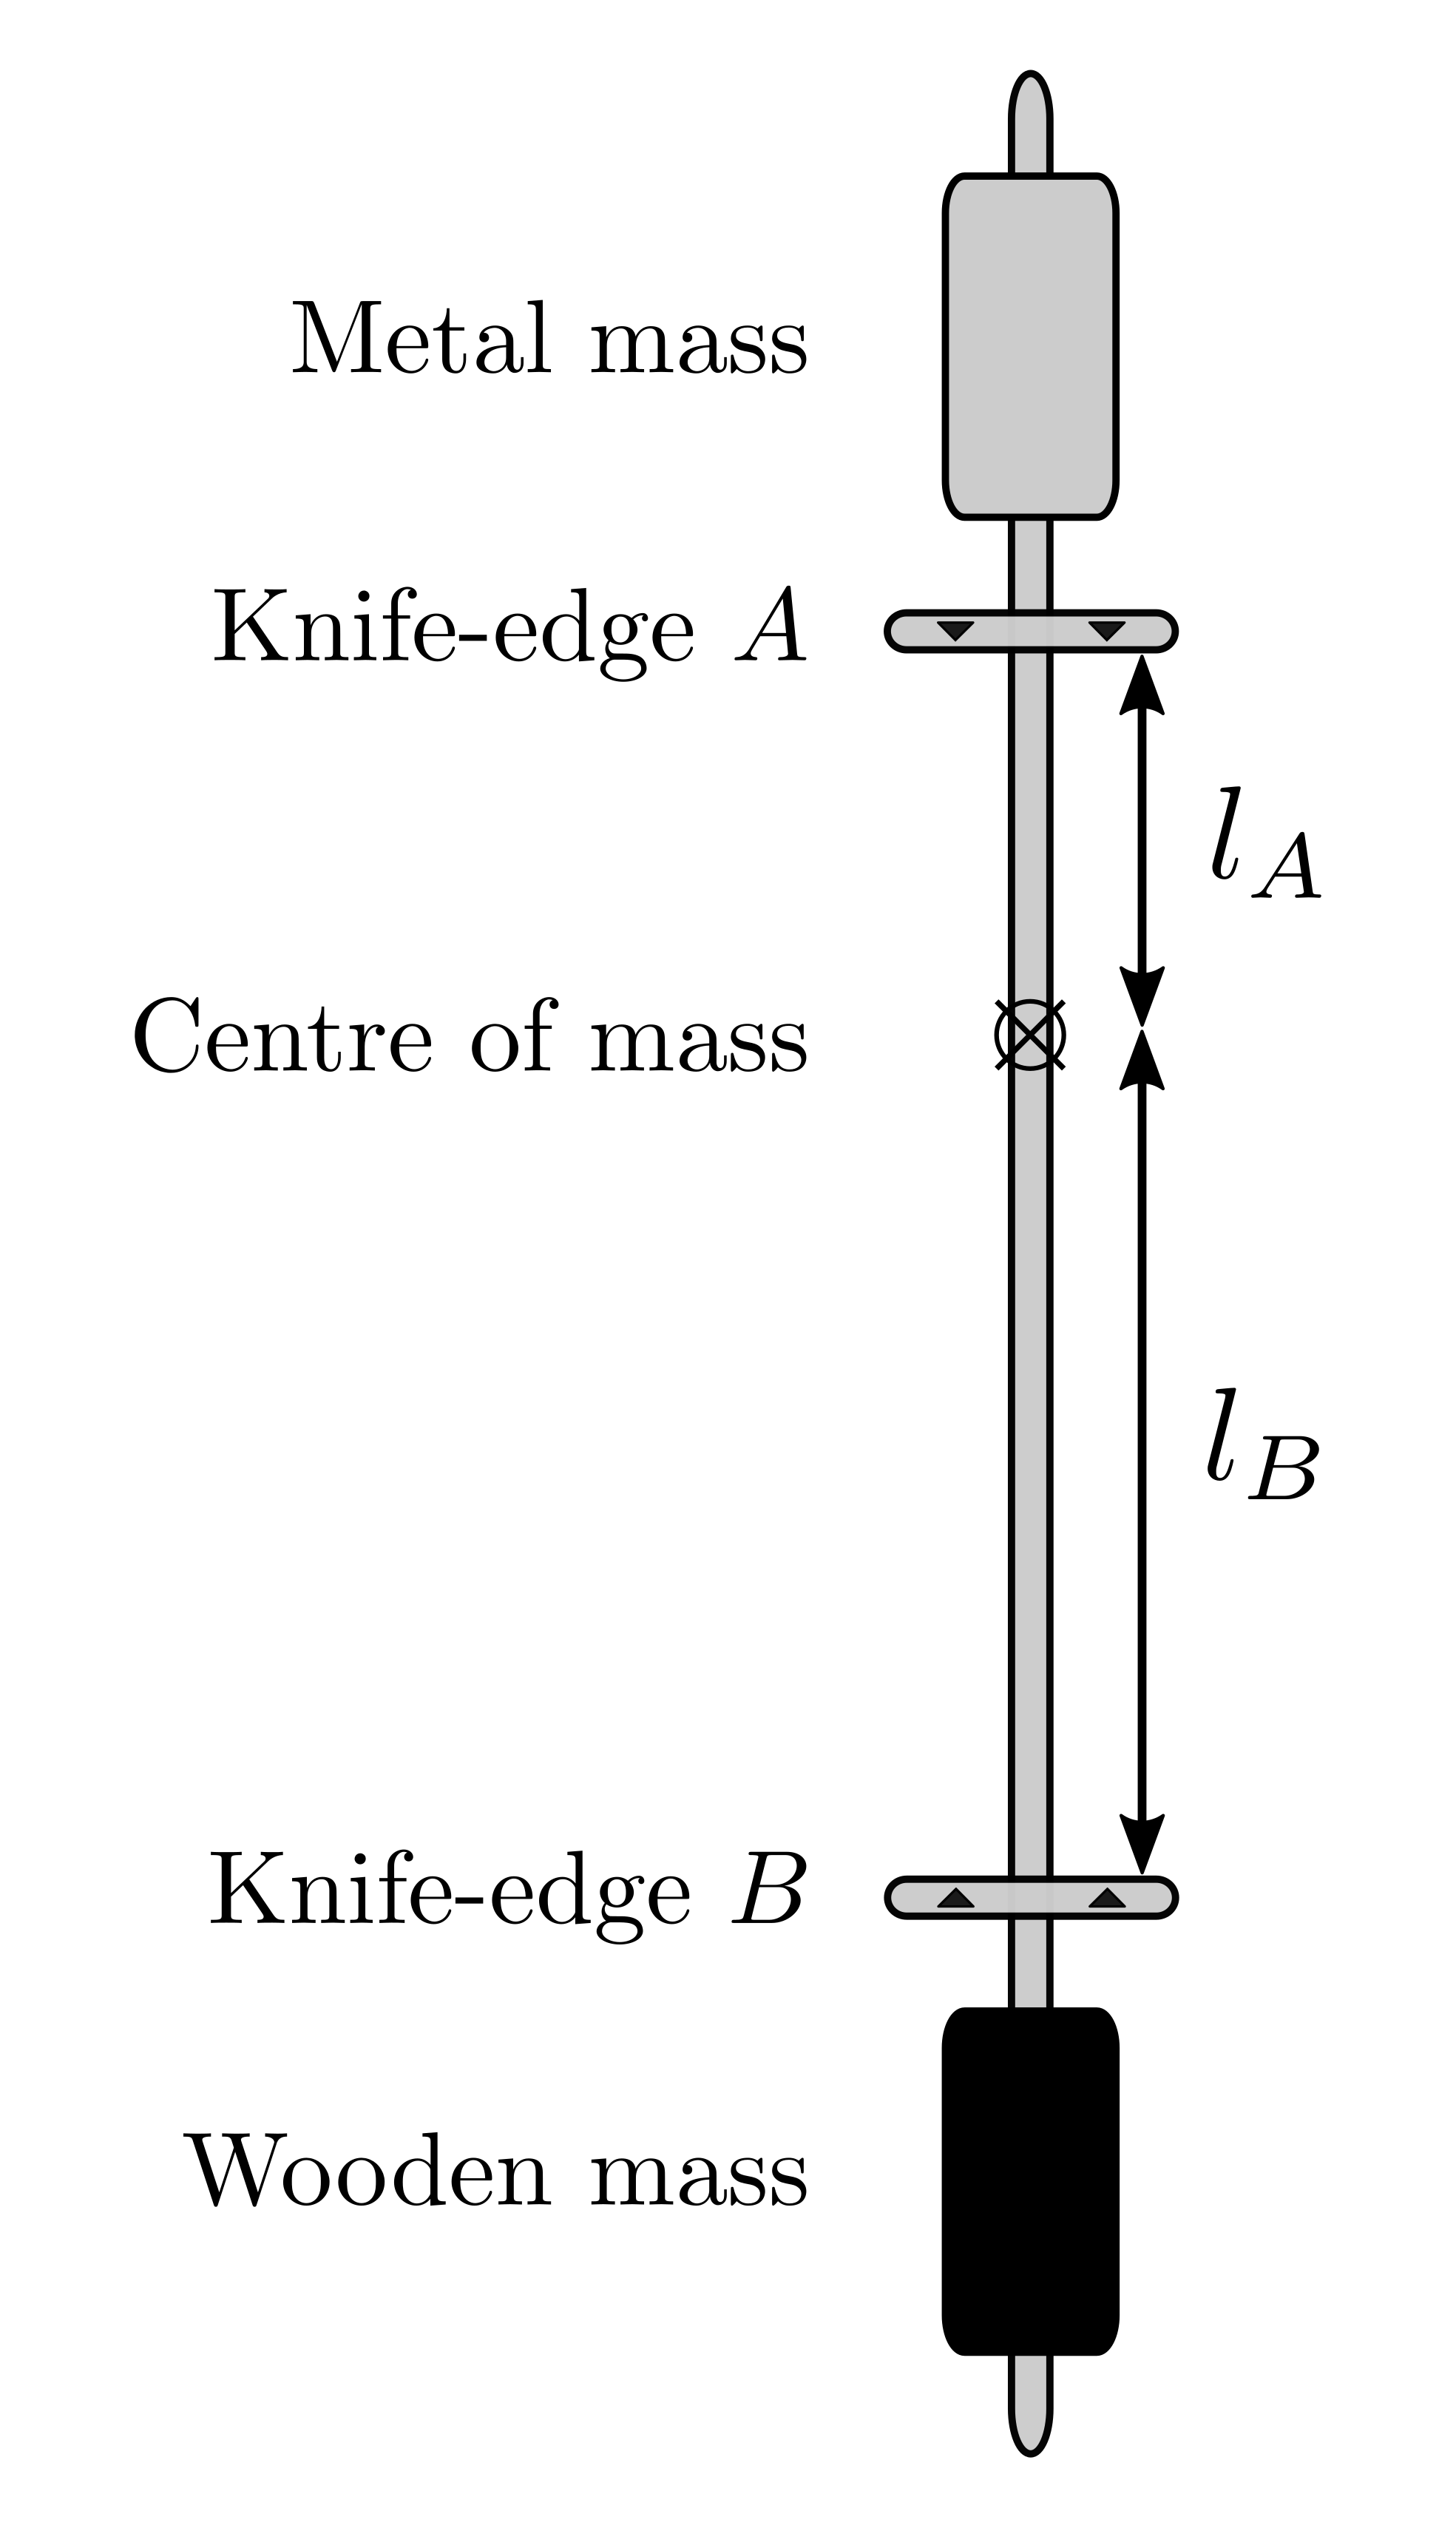
\includegraphics[scale=0.4]{figs/katers-pendulum/katers-setup.png}
        \caption{Schematic of the Kater's pendulum set-up. The pendulum is composed of a thick rod with two knife edges that allow it to be suspended from either end. Two unequal masses are placed on either side, and can be moved along the rod if necessary.}
        \label{fig:katers-setup}
\end{figure}

   
Consider the oscillations of such a pendulum in two different configurations:
\vspace{-\parskip}
\begin{enumerate}
    \item First, consider the pendulum suspended at the knife edge $A$, at a distance $l_A$ from the centre of mass, with some period of oscillation $T_A$.
    \item Next, consider the pendulum suspended about knife edge $B$, at a distance $l_B$ from the centre of mass, with some period of oscillation $T_B$.
\end{enumerate}

In each of the above cases, we can use the equation for the time-period of a compound pendulum and the parallel axis theorem -- Equations~(\ref{eq:Tcomp}) and~(\ref{parallel-axis-theorem}) respectively -- to relate the time period to the different parameters in the problem. In particular, if we denote the total mass of the pendulum $m$, we have
\begin{equation}
    \begin{aligned}
    T_A&=2\pi\sqrt{ \frac{I_{CM}+ m\,l_A^2} {m\,g\,l_A} },\\
    T_B&=2\pi\sqrt{ \frac{I_{CM}+ m\,l_B^2} {m\,g\,l_B} }.
    \end{aligned}
\end{equation}
We can eliminate $I_{CM}$ from the above equations, to get
\begin{equation}
    \frac{1}{g}=\frac{1}{4\pi^2} \left(\frac{T_A^2+T_B^2}{ 2(l_A+l_B)}+\frac{T_A^2-T_B^2}{ 2(l_A-l_B)} \right).
    \label{eqn:full-katers-g}
\end{equation}

Thus, we have managed to circumvent the issue of knowing the exact mass distribution of the pendulum, since we have a formula for $g$ that does not depend on the moment of inertia of our pendulum.

However, a further problem remains: in the second term above, we need to find $l_A - l_B$. This requires us to know the exact location of the centre of mass, which is difficult to measure precisely. We would thus like to eliminate this second term. We do this by realising that if we are able to choose our parameters such that $T_A = T_B$, the entire term will be set to zero. We know that that is a possibility because for any compound pendulum, there are two distances with the same oscillation period. The asymmetric mass distribution pushes the centre of mass away from the geometrical centre of the pendulum, and allows two conjugate points of suspension to be accessible.

% \begin{question}
% \textbf{Question:} Can you show why in this case $T_A = T_B$, but $l_A \neq l_B$?
% \end{question}

Thus, when we find the pivot points with same time periods, $T_A = T_B = T$, we can simplify the expression for $g$ to
\begin{equation}
    g = 4\pi^2 \left(\frac{l_A + l_B}{T^2}\right),
    \label{eqn:g-TA=TB}
\end{equation}

which provides us an accurate measurement of the acceleration due to gravity $g$ that does not require knowing either the mass distribution \textsl{or} the location of the centre of mass!

\begin{question}
\textbf{Question:} In the above formula, $l_A + l_B$ seems like the sum of two separate lengths measured with respect to the centre of mass. Experimentally, is this truly the sum of two lengths? 

\textbf{Question:} An important approximation of Equation~(\ref{eqn:full-katers-g}), probably derived by Bessel, is very useful to show that the expression for $g$ is much less sensitive to the location of the centre of mass, if $T_A = T_B$. Defining $T= (T_A + T_B)/2$, $\Delta T = (T_A - T_B)$, and $L=l_A + l_B$, show that if you ignore higher powers of $\Delta T$, $g$ can be very accurately approximated as
\begin{equation}
    g = \frac{8 \pi^2}{\dfrac{T_A^2 + T_B^2}{l_A + l_B} + \dfrac{T_A^2 - T_B^2}{l_A - l_B}} \approx \frac{4 \pi^2 L}{T^2} \left( 1 + \left( \frac{\Delta T}{T} \frac{L}{L-2l_A} \right)\right).
    \label{eqn:simplified-g}
\end{equation}
\end{question}

 
\section*{Experimental Setup}

\subsection*{Apparatus}

\begin{enumerate}
\itemsep0em
    \item A reversible Kater's Pendulum and a wall mount
    \item Assorted wooden and metal weights
    \item A stopwatch 
    \item A heavy wedge with which to determine the centre of mass of the pendulum rod
\end{enumerate}


\subsection*{Precautions}
\begin{itemize}
\itemsep0em
    \item The pendulum system is very heavy, make sure you do not drop it on your (or rather, anyone's) feet.
    
    \item The pendulum can be a spear. Make sure you carry it such that it does not hurt anyone.
    
    \item Make sure the knife edges are tightened (using a pair of pliers) to ensure that they do not slide during oscillations.
    
    \item The wooden weight has a tendency of slipping even when the screw is tightened by a pair of pliers. As a result, you might want to mark the position of the wooden block to keep track of it in case it moves. 
\end{itemize}


\section*{Procedure}

\subsection*{Part A}

You will begin this experiment by using the rod of the Kater's pendulum as a compound pendulum, and try to find four points on it which have the same time period $T$.

\begin{enumerate}
\itemsep0em
    \item Take the rod of the pendulum and a single knife-edge. Measure the centre of mass of the rod using a heavy wedge.
    
    \begin{question}
    \textbf{Question:} What is the radius of gyration $k$ of a rod of mass $M$? Assume the rod to be cylindrical; you will need to calculate its moment of inertia, and then use the definition of the radius of gyration.
    \end{question}
    
    \item Attach the knife-edge at one end of the rod, at some distance $l$ from the centre of the rod, and measure the time-period for 10 oscillations.
    
    \item Change $l$ by moving the knife-edge from one of the rod to the other, and measure the time period for 10 oscillations in each case.\
    
    \begin{imp}
    Ensure that the centre of mass is always below the knife-edge or the pendulum will topple over. You can do this by flipping the knife-edge as you cross the centre of mass.
    \end{imp}
    
    \item Plot a graph of $T$ vs. $l$, and show that there are four points which have the same time period. 
    
    \begin{question}
    \textbf{Question:} Why do we not need to take the moment of inertia of the knife-edge into account in this case?
    \end{question}
\end{enumerate}

\subsection*{Part B}

Next, you will use Kater's pendulum -- as it was intended -- to determine the local acceleration due to gravity $g$.

\begin{enumerate}
\itemsep0em
    \item Mark the centre of the rod and fix the masses at some fixed distance $d$ from this centre.
    
    \item Fix both the knife-edges some distance apart (call this $l$) on either side of the centre of the rod.
    
    \item By moving both masses with respect to their knife edges (i.e.\ the configuration of the system), change the centre of mass of the system. For each such position, measure $T_A$ and $T_B$ for 10 oscillations, and make a table of $T_A - T_B$, making sure you keep track of the sign. 
    
    \item You will notice that $T_A - T_B$ will change from positive to negative, thus indicating the configuration for which $T_A = T_B$. (Make sure you note down both $l_A + l_B$ and $l_A - l_B$.)

    \item Move to this configuration, and measure $T_A$ and $T_B$ again for 10 oscillations. If the difference is significant, make small adjustments until $T_A$ and $T_B$ are as close to each other as you can make them. One you have decided on your final configuration, measure $T_A$ and $T_B$ for 100 oscillations, making sure you count your oscillations carefully. 
    
    \begin{tip}
    If you make a mistake in counting the oscillations, this will show up in a comparison of the time periods obtained from 10 oscillations and those obtained from 100 oscillations.
    \end{tip}

\end{enumerate}

\subsection*{Part C}

Finally, you will perform a detailed analysis of the uncertainties on your result. 

\begin{imp}
There is a reason that the analysis of uncertainties in this experiment takes up an entire part of the experiment: it is extremely involved. Please make sure you pay attention to doing it well.
\end{imp}

For this analysis, it is essential to use the measured variables $T_A, T_B, L,$ and the larger length (say, $l_A$).

\begin{question}
\textbf{Question:} Why do you not need to use $l_B$ for the error analysis?

\textbf{Question:} Why is the \textsl{larger} length $l_A$ chosen?
\end{question}


\begin{enumerate}
    \item We begin with a result from uncertainty analysis: if a physical quantity $q$ is a function of multiple variables, i.e. $q = f(x,y,z)$, then the net uncertainty in $q$ -- which we denote $\Delta q$ -- can be computed using the formula
    \begin{equation}
        \Delta q^2 = \left(\pdv{f}{x}\right)^2 \Delta x^2 + \left(\pdv{f}{y}\right)^2 \Delta y^2 + \left(\pdv{f}{z}\right)^2 \Delta z^2.
    \end{equation}

    The above equation is just saying that the independent uncertainties due to the variables $x,y,$ and $z$ add in \textsl{quadrature}.
    
    \item Argue that the uncertainty in $g$ can thus be computed using the partial derivatives $$\pdv{g}{T_A},\quad \pdv{g}{T_B},\quad \pdv{g}{L},\quad \text{and} \quad \pdv{g}{l_A}.$$
    \begin{question}
        \textbf{Question:} In order to compute these derivatives, you should use Equation~(\ref{eqn:simplified-g}) and not the simpler Equation~(\ref{eqn:g-TA=TB}). Why?
        \textbf{Hint:} What assumption has been made when deriving Equation~(\ref{eqn:simplified-g})? 
    \end{question}

    \item Identify the uncertainties $\Delta T_A$, $\Delta T_B$, $\Delta L$, and $\Delta l_A$. Use these uncertainties to compute the error in $g$.
\end{enumerate}

